\documentclass[10pt,twocolumn,letterpaper]{article}

\usepackage{cvpr}
\usepackage{times}
\usepackage{epsfig}
\usepackage{graphicx}
\usepackage{amsmath}
\usepackage{amssymb}
\usepackage[utf8]{inputenc}
\usepackage{booktabs,tabularx,enumitem,ragged2e}
\usepackage{subcaption}

% Include other packages here, before hyperref.

% If you comment hyperref and then uncomment it, you should delete
% egpaper.aux before re-running latex.  (Or just hit 'q' on the first latex
% run, let it finish, and you should be clear).
\usepackage[breaklinks=true,bookmarks=false]{hyperref}

\cvprfinalcopy % *** Uncomment this line for the final submission

\def\cvprPaperID{****} % *** Enter the CVPR Paper ID here
\def\httilde{\mbox{\tt\raisebox{-.5ex}{\symbol{126}}}}

% Pages are numbered in submission mode, and unnumbered in camera-ready
%\ifcvprfinal\pagestyle{empty}\fi
\setcounter{page}{1}

\begin{document}

%%%%%%%%% TITLE
\title{Project Report: Scan2Cap}

\author{
\small Felix Wimbauer\\
\small Technical University of Munich\\
{\tt\small felix.wimbauer@tum.de}
% For a paper whose authors are all at the same institution,
% omit the following lines up until the closing ``}''.
% Additional authors and addresses can be added with ``\and'',
% just like the second author.
% To save space, use either the email address or home page, not both
\and
\small Nicolas Seppich\\
\small Technical University of Munich\\
{\tt\small nicolas.seppich@tum.de}
\and
\small
\textbf{Supervisor}: Dave Zhenyu Chen\\
\small
Technical University of Munich\\
{\tt\small zhenyu.chen@tum.de }
}

\maketitle
%\thispagestyle{empty}

%%%%%%%%% ABSTRACT
\begin{abstract}
In this work, we investigate the task of generating a description for a target object in context to its environment in the 3D domain. To this end, we propose a pipeline which combines concepts from 3D object detection and visual attention-based captioning. The proposed pipeline first uses VoteNet to extract feature vectors of the scene. It then combines this information with the features of the object of interest, which are extracted by PointNet++, and feeds this data into an LSTM captioning mechanism, that generates a caption of the object in context of the scene.\\{\normalfont{\footnotesize \texttt{
\textbf{Links}: \href{https://youtu.be/RB6qlZPY2iM}{Presentation Video}, \href{https://gitlab.lrz.de/wimbauer/adl4cv}{Gitlab Repository}}}}
\end{abstract}

%%%%%%%%% BODY TEXT
\section{Problem Statement \& Motivation}

Extracting a detailed and correct description of a 3D scene and included objects is crucial for many tasks, e.g. in robotics for navigation and interaction with objects.
However, to the best of our knowledge, there has been no work so far to generate a description of an object representation in point clouds or 3D data. Therefore, we are interested in implementing a pipeline to obtain a description for a given object in a 3D scan to place it into a global semantic context within its environment. This project lays down the groundwork for dense captioning, in which you compute a caption for all objects in that scene.
 
%-------------------------------------------------------------------------
\section{Related Work}
Our work is based on the ScanRefer \cite{chen2019scanrefer} dataset and reference implementation for object relocalization. The dataset consists of 1513 RGB-D scans of ScanNet \cite{dai2017scannet} and contains approximately 5 unique object descriptions for each object in each scene. The extraction of features on point clouds is presented by \cite{qi2017pointnet++}, who apply the feature extraction directly on the point cloud on a hierarchical level, allowing the extraction of local features in a global context. The architecture has also been extended to object detection in \cite{qi2019deep}. Methods for image captioning using visual attention are described by \cite{xu2015show}, \cite{lu2017knowing} and \cite{anderson2018bottom}.

%-------------------------------------------------------------------------
\section{Architecture}

Given a point cloud $\mathit{p \in R^{N\times(d+C)}}$ and an object in that scene, which is described by a target bounding box $b_{target}\in R^6$, our goal is to generate a meaningful caption for the object embedded in the context of the scene. To this end, we used three different pipelines, which are described in the following.

\begin{figure*}	
	\centering
	\begin{minipage}[b]{.55\textwidth}
		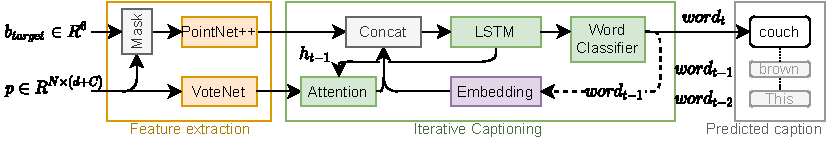
\includegraphics[width=.95\textwidth]{figures/arch_condensed_2.pdf}
		\caption{Attention-based architecture}
		\label{fig:arch}
	\end{minipage}
	\begin{minipage}[b]{.44\textwidth}
		{\scriptsize 
			\begin{tabular}{|l|cccc|}
			\hline
			\textbf{Model} & \textbf{BLEU-4} & \textbf{ROUGLE-L} & \textbf{METEOR} & \textbf{CIDEr}\\
			\hline
			Baseline & 0.434 & 0.569 & 0.617 & 0.692 \\
			With VoteNet & \textbf{0.447} & 0.580 & 0.625 & 0.757 \\
			With Attention & 0.447 & \textbf{0.584} & \textbf{0.626} & \textbf{0.792} \\
			\hline
		\end{tabular}}
		\vspace{.5\baselineskip}
		\captionof{table}{Quantitative results}
		\label{tab:quantitative_results}
	\end{minipage}
\end{figure*}

\subsection{Baseline}

To extract information from the point cloud, we use a PointNet++ \cite{qi2017pointnet++} model. To give the network information about which object we are interested in, we add a new feature channel to each point that masks all points that lay within the bounding box of the object. To ensure that we receive meaningful features, we use weights pretrained for classification of the masked object.

To generate the caption, we use a classical LSTM with an appended fully-connected layer. The fully-connected layer acts as a word classifier and maps the hidden state $h_{t}$ of the LSTM to our vocabulary. As input, the LSTM receives the feature vector extracted from the point cloud and the word embedding vector of the previously generated word. The word embedding is taken from a pre-computed GloVe \cite{pennington2014glove} word embedding matrix. This structure of the iterative caption generation is similar to \cite{xu2015show}.

\subsection{Better Feature Extraction with VoteNet}

Because the PointNet++ feature vector contains mostly object specific and not global features, the baseline approach is limited. In the second architecture iteration, we therefore employ a VoteNet \cite{qi2019deep} network, which computes a fixed number of object proposals and according feature vectors for our point cloud. Those feature vectors help the network to understand the surroundings of the object we want to describe. Because the number of proposals may vary and the proposals are not in a fixed order, we average pool them to obtain a concise representation of the information. This pooled feature vector is finally concatenated with the feature vector from PointNet++ and the embedding vector of the previously predicted word to then be passed into the LSTM.

\subsection{Better Captioning with Attention}

Average pooling the feature vectors from VoteNet is not ideal as often only a small number of the object proposals is relevant for the final caption. Therefore, in the third model iteration we replace the average pooling step from before with an attention mechanism, as it is described in \cite{xu2015show}. The attention mechanism receives the hidden state of the captioning LSTM from the previous iteration and the feature vectors of the object proposals. It then predicts a weighting for the different object proposals and pools the feature vectors based on those weights. This approach allows our model to select the most relevant object for each token in the caption and make word predictions that better match the the context of the scene. This architecture is shown \autoref{fig:arch}.


\section{Experiments \& Results}

In our experiments, we use the same training pipeline for our three models. Similar to \cite{xu2015show}, all architectures make use of teacher-forcing during training: instead of inserting the previous predicted word, the LSTM receives the previous ground truth word as input for captioning along with the encoded feature vectors of the scene. This allows for faster convergence by minimizing drift between the ground truth token and predicted word in training time. In evaluation time, the network takes the previously predicted word as input. During experiments, we found that our models based on VoteNet performed best when we filter out all objects that have an objectness score value below 0.75 and use only the 8 closest objects.

As metrics for performance evaluation we rely on BLEU \cite{Papineni2002BleuAM}, ROUGE-L \cite{Lin2004ROUGEAP}, METEOR \cite{Denkowski2014MeteorUL} and CIDEr \cite{DBLP:journals/corr/VedantamZP14a}.  In this paper we focus on the BLEU-4 score to determine the best models as in \cite{xu2015show}. 

\subsection{Quantitative Improvements}
In this experiment, we investigate the influence of the architectural improvements we propose. All models include the same pre-trained masked PointNet++ feature extractor. 
\hyperref[tab:quantitative_results]{Table~\ref*{tab:quantitative_results}} shows the quantitative results. 

Firstly, the baseline model achieves fairly good results that are not far from the improved architectures. Comparing the BLEU-4 score to the results of the COCO Image Captioning Challenge 2015 \cite{COCO}, our models outperform the best-performing architectures. However, we argue that our vocabulary and gt sentence structure is much simpler and therefore leads to better scores.

Secondly, the results show that improving the feature extraction (VoteNet) and the captioning mechanism (attention) leads to higher scores. The best results are obtained by the attention model, except for the BLEU-4 score where the improved architecture is marginally better.                

\subsection{Qualitative Analysis}
In this experiment, we analyze the quality of the predicted descriptions in two examples \autoref{fig:examples}. 
The first example shows the comparison between the predictions of our three architectures. The three models predict a reasonable description but differ slightly in the conceived context. The attention model is able to make the most context-specific prediction by focusing on the bed (visible through color coding), a very unusual combination. This is also visible in the second example. Additionally, we can observe that our network relies on a simple two sentence-structure. We believe that this is a result of the distribution of the ScanRefer data set. Analysis of the number of tokens per description shows that the distribution of predicted and ground truth captions share the same mode of 15 tokens, however, the predicted captions have a smaller mean and variance.

\begin{figure}[b]
	\centering
	\begin{subfigure}[c]{.49\linewidth}
		\centering
		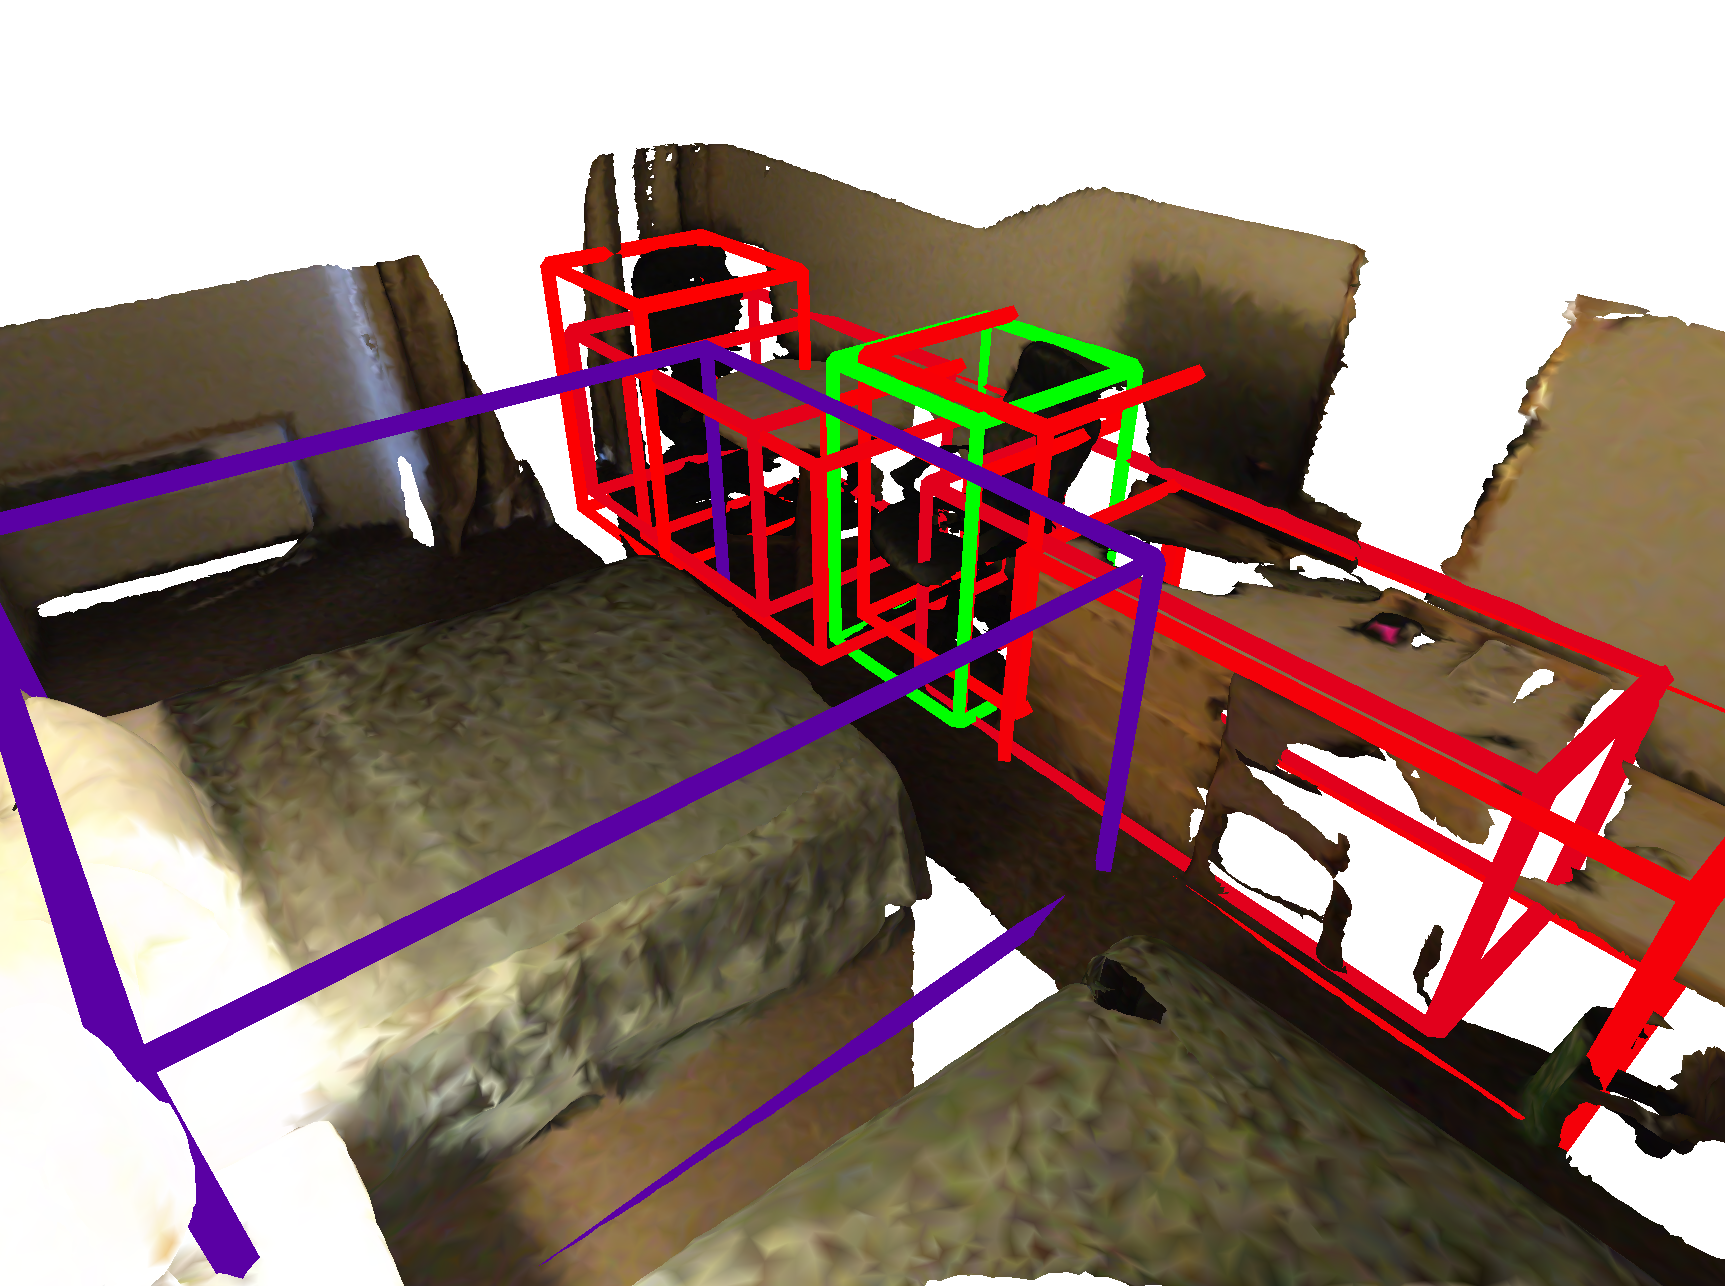
\includegraphics[width=\linewidth]{figures/gt_scene0221_00_3_0_att_noshade.png}
		\label{fig:example_1}
	\end{subfigure}
	\begin{subfigure}[c]{.49\linewidth}
		\centering
		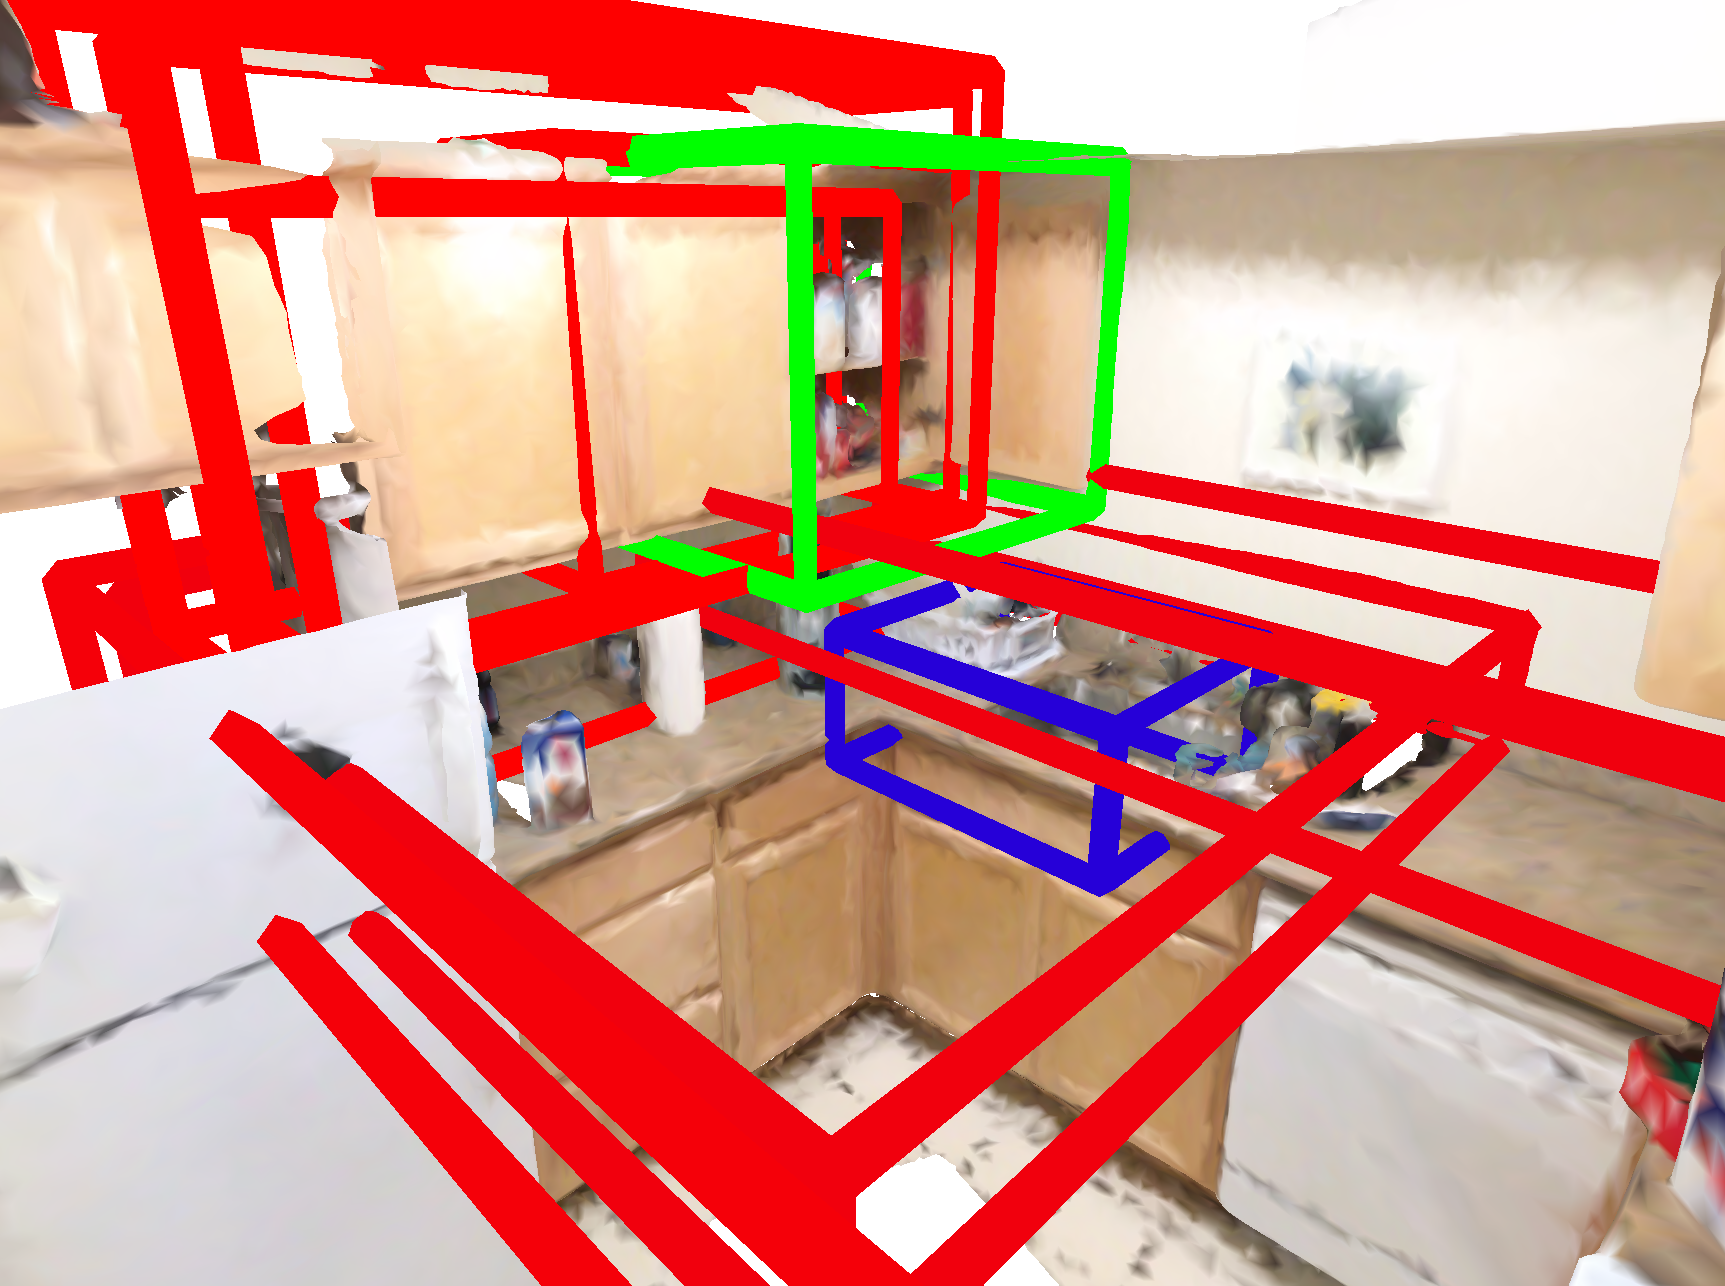
\includegraphics[width=\textwidth]{figures/gt_scene0164_00_2_0_att_noshade.png}
		\label{fig:example_2}
	\end{subfigure}
	\vspace{-1.\baselineskip}
	\begin{flushleft}
		{\scriptsize 
			\textit{Left image:}\\
			\textbf{GT}: there is a black chair. it is next to a cabinet on the side of the room .\\
			\textbf{BL}: this is a black chair . it is to the left of the table .\\
			\textbf{VN}: this is a black chair . it is to the left of the desk .\\
			\textbf{Att}: this is a black chair . it is at the end of the \underline{bed} .\\
			\vspace{.5\baselineskip}
			\textit{Right image:}\\
			\textbf{GT}: the open kitchen cabinet is directly above the sink and the water container. the open kitchen cabinet is a brown box with one side hanging out .\\
			\textbf{Att}: this is a white kitchen cabinet . it is above the \underline{sink} .\\
			\textbf{Legend}: \textbf{GT}-Groundtruth, \textbf{BL}-Baseline, \textbf{VN}-With VoteNet, \textbf{Att}-With Attention \textbf{Bounding boxes}: \textbf{\color{green} Green}-Target object, \textbf{{\color{red}Red}-{\color{blue}Blue}}-Lowest to highest attention for marked token
		}
	\end{flushleft}
	\vspace{-1.\baselineskip}
	\caption{Examples from the ScanRefer validation set}
	\label{fig:examples}
\end{figure}

{\small
\bibliographystyle{ieee_fullname}
\bibliography{report}
}

\end{document}
